\documentclass[10pt,twocolumn]{article}

% use the oxycomps style file
\usepackage{oxycomps}


% usage: \fixme[comments describing issue]{text to be fixed}
% define \fixme as not doing anything special
\newcommand{\fixme}[2][]{#2}
% overwrite it so it shows up as red
\renewcommand{\fixme}[2][]{\textcolor{red}{#2}}
% overwrite it again so related text shows as footnotes
%\renewcommand{\fixme}[2][]{\textcolor{red}{#2\footnote{#1}}}

% read references.bib for the bibtex data
\bibliography{references}

% include metadata in the generated pdf file
\pdfinfo{
    /Title (Exploring Unsupervised Clustering and Analysis of Bot Behavior on Twitter Using NLP and Metadata)
    /Author (Karlo Papa)
}


% set the title and author information
\title{Exploring Unsupervised Clustering and Analysis of Bot Behavior on Twitter Using NLP and Metadata}
\author{Karlo Papa}
\affiliation{Occidental College}
\email{kpapa@oxy.edu}

\begin{document}

\maketitle

\section{Introduction}

The proliferation of automated accounts, or bots, on social media platforms has become a growing concern for researchers and the public. Bots serve a variety of purposes, from benign uses such as automated posting and customer service to malicious activities like disinformation, spam, and social engineering campaigns. Recent studies also warn that large language models are lowering the barrier for attackers to spin up highly convincing AI-generated personas~\cite{Adams2017ai,Yu2024the}. Detecting and understanding the behaviors of these bots is critical to preserving the integrity of online discourse.

Twitter has become a primary platform for bot detection research, given its open data access and widespread use across political, business, entertainment, and social domains. Bots on Twitter vary in sophistication: while some are easily detected spam bots, others engage in subtle manipulation and imitation of human users. Traditional supervised learning approaches, such as Random Forests and Support Vector Machines (SVM), have been widely adopted due to their accuracy on labeled data. However, these methods rely on the availability of high-quality labels, which are costly and time-consuming to obtain. Furthermore, supervised models may struggle to detect emerging and sophisticated bot behaviors that differ from previously labeled examples.

Unsupervised methods offer an alternative, potentially uncovering structure in unlabeled data and identifying new bot behaviors. This project investigates the utility of unsupervised learning, enhanced with natural language processing (NLP) and metadata features, for bot detection. Through experiments on the Cresci bot dataset, I applied K-Means, Agglomerative Clustering, ensemble clustering, and dimensionality reduction methods. These methods demonstrated moderate clustering success, with ensemble clustering achieving up to 72\% unsupervised accuracy on labeled clusters. To complement this analysis, I trained a supervised Random Forest model, which achieved near-perfect classification results, validating the power of the combined feature set.

Ultimately, this work aims to bridge unsupervised and supervised methods to better understand bot behaviors, reduce reliance on costly labels, and contribute to more adaptable detection systems. I’m drawn to this project because it combines my interest in machine learning with pressing societal concerns like misinformation and online safety. Methodologically, the project spans clustering, classification, dimensionality reduction, and behavioral analysis—making it both technically rigorous and interdisciplinary. Its scope and complexity are well-matched to the Oxy CS senior comprehensive project.


\section{Technical Background}

Bots on social media vary widely in their behavior and sophistication. While some attempt to mimic human interactions by retweeting, replying, or posting plausible text, others are easily detectable through repetitive posting, unusually high activity levels, or minimal engagement with other users~\cite{ferrara2016rise,cresci2017paradigm}. These behavioral signals form the foundation of many machine learning-based detection systems.

Historically, bot detection has relied on supervised learning. Classifiers trained on labeled datasets leverage metadata (such as follower counts and retweet frequencies) and linguistic features (such as text style and sentiment) to distinguish between bots and humans~\cite{varol2017online}. Although effective in many cases, supervised models face significant challenges. Labeled datasets are expensive to curate and can quickly become outdated as bot developers continuously adapt their strategies. Moreover, supervised models inherently struggle to detect novel or subtle forms of automation that differ from previously observed patterns.

Unsupervised learning offers a promising alternative. Rather than relying on labels, clustering algorithms such as K-Means and Agglomerative Clustering aim to automatically group similar users based on patterns in their behavior and language. The goal is to reveal natural groupings—such as botnets or coordinated campaigns—that may not yet be captured in labeled data. However, applying clustering to social media is difficult. Text data in particular is high-dimensional and sparse, making it challenging to compute meaningful similarities between users. 

To address this, dimensionality reduction and natural language processing (NLP) techniques are commonly employed. Early explorations on Instagram~\cite{Akyon2019instagram} and controlled user-studies on deception detection~\cite{Kenny2022duped} underline how feature choice can drastically shift clustering outcomes. Principal Component Analysis (PCA) reduces the number of features while preserving the most informative variance, and t-SNE is used to preserve local relationships in complex data for visualization and clustering~\cite{van2008visualizing}. Complementing these methods, TF-IDF (Term Frequency-Inverse Document Frequency) vectorization transforms tweet content into numerical features that capture the importance of words across different accounts. When combined with metadata, these techniques produce compact and informative feature representations that make unsupervised clustering more effective.

This project builds on these foundations by combining TF-IDF-based linguistic features and account-level metadata, reducing the dimensionality of this data, and applying clustering algorithms to detect patterns without supervision. The same feature set is also used in supervised classification experiments to benchmark unsupervised results and explore hybrid detection strategies. Together, these techniques form the core methodology for analyzing and detecting bots with greater flexibility and interpretability.


\section{Prior Work}
Bot detection has been extensively studied through
various machine learning approaches, each with distinct
strengths and limitations. However, much of the existing
work focuses on detecting easily identifiable spam and dis-
information bots, raising questions about how well these
models generalize to more subtle and socially engineered
bot behaviors.

\subsection{Strengths and Limitations of Researched Models} 
Early work frames bot detection as a standard binary‐classification problem. Random Forests and Support Vector Machines (SVMs) perform well when high-quality labels are available, routinely surpassing 90\% accuracy on benchmark datasets~\cite{Heidari2021empirical,varol2017online,Hayawi2023social}.  
These studies extract rich metadata features—follower counts, tweet rates, URL ratios—and simple linguistic cues to flag spam or political-influence bots. Replication papers, however, show that public datasets over-represent obvious spam or election campaigns~\cite{cresci2017paradigm,Orabi2020detection}.  Models trained on such skewed labels struggle with subtler social-engineering accounts and require continual retraining as bot tactics evolve.

To reduce label dependence, several authors employ clustering (K-Means, DBSCAN) and anomaly detectors (Isolation Forest) to surface suspicious accounts without prior annotation~\cite{Grimme2018changing,Orabi2020detection}.  
While these methods can expose botnets at scale, validation is difficult: clusters frequently mix sophisticated bots with fringe—but legitimate—users, and Adjusted Rand Index (ARI) scores rarely exceed 0.25 on held-out labels~\cite{Yang2023anatomy}.  These findings set a realistic target for my own clustering experiments and justify exploring ensemble clustering to boost precision.

A parallel thread embraces deep learning. Long Short-Term Memory (LSTM) and Convolutional Neural Network (CNN) models capture temporal and stylistic patterns beyond hand-crafted features and deliver strong F1 scores on text-rich datasets~\cite{Cai2017behavior,Kudugunta2018deep}.  
However, they demand thousands of labeled examples, incur heavy compute costs, and offer limited interpretability~\cite{Wei2020twitter}.  The recent wave of large language models capable of writing human-like tweets further erodes their robustness, as detectors tuned on older data misclassify these AI-generated bots. This further underscores the need for continuously adaptive methods.

Recognizing that no single technique suffices, recent work layers methods—e.g., clustering to propose candidates followed by a lightweight classifier, or semi-supervised pseudo-labeling loops—to combine high recall with acceptable precision~\cite{Hayawi2023social,Mbona2023classifying}.  Such hybrids consistently outperform individual models and point toward adaptive, multi-view systems.

\subsection{Takeaways for This Project} 
Taken together, the literature suggests that (i) supervised models excel yet drift with label bias, (ii) pure clustering is informative but noisy, and (iii) integrating metadata, text, and temporal cues in hybrid pipelines offers the most resilient path.  
Guided by these insights, my three-week prototype applied K-Means, Agglomerative, and a Random Forest baseline, then formed a small ensemble that exceeded either clusterer alone.  My proposed fall work will expand this hybrid into an interpretable, semi-supervised pipeline better suited to the rapidly evolving landscape of AI-generated bots.


\section{Three-Week Project and Results}

The three-week project served as a foundational exploratory phase for my broader comps project, with the goal of developing a deeper understanding of unsupervised bot detection and validating potential of hybrid methods. While the long-term objective is to create a flexible detection framework that combines unsupervised discovery with supervised classification, this initial stage focused on experimentation and analysis to assess feasibility.

\subsection{Project Workflow}

The project began by preparing and processing the Cresci 2017 bot dataset~\cite{cresci2017paradigm}, which includes various types of bot and genuine accounts. I extracted both metadata features (e.g., follower counts, posting frequency) and tweet content, which was transformed into numerical representations using TF-IDF vectorization. To address the high dimensionality of the data, Principal Component Analysis (PCA) and t-SNE were employed to reduce the feature space~\cite{van2008visualizing} and improve clustering performance.

\begin{figure}[ht]
    \centering
    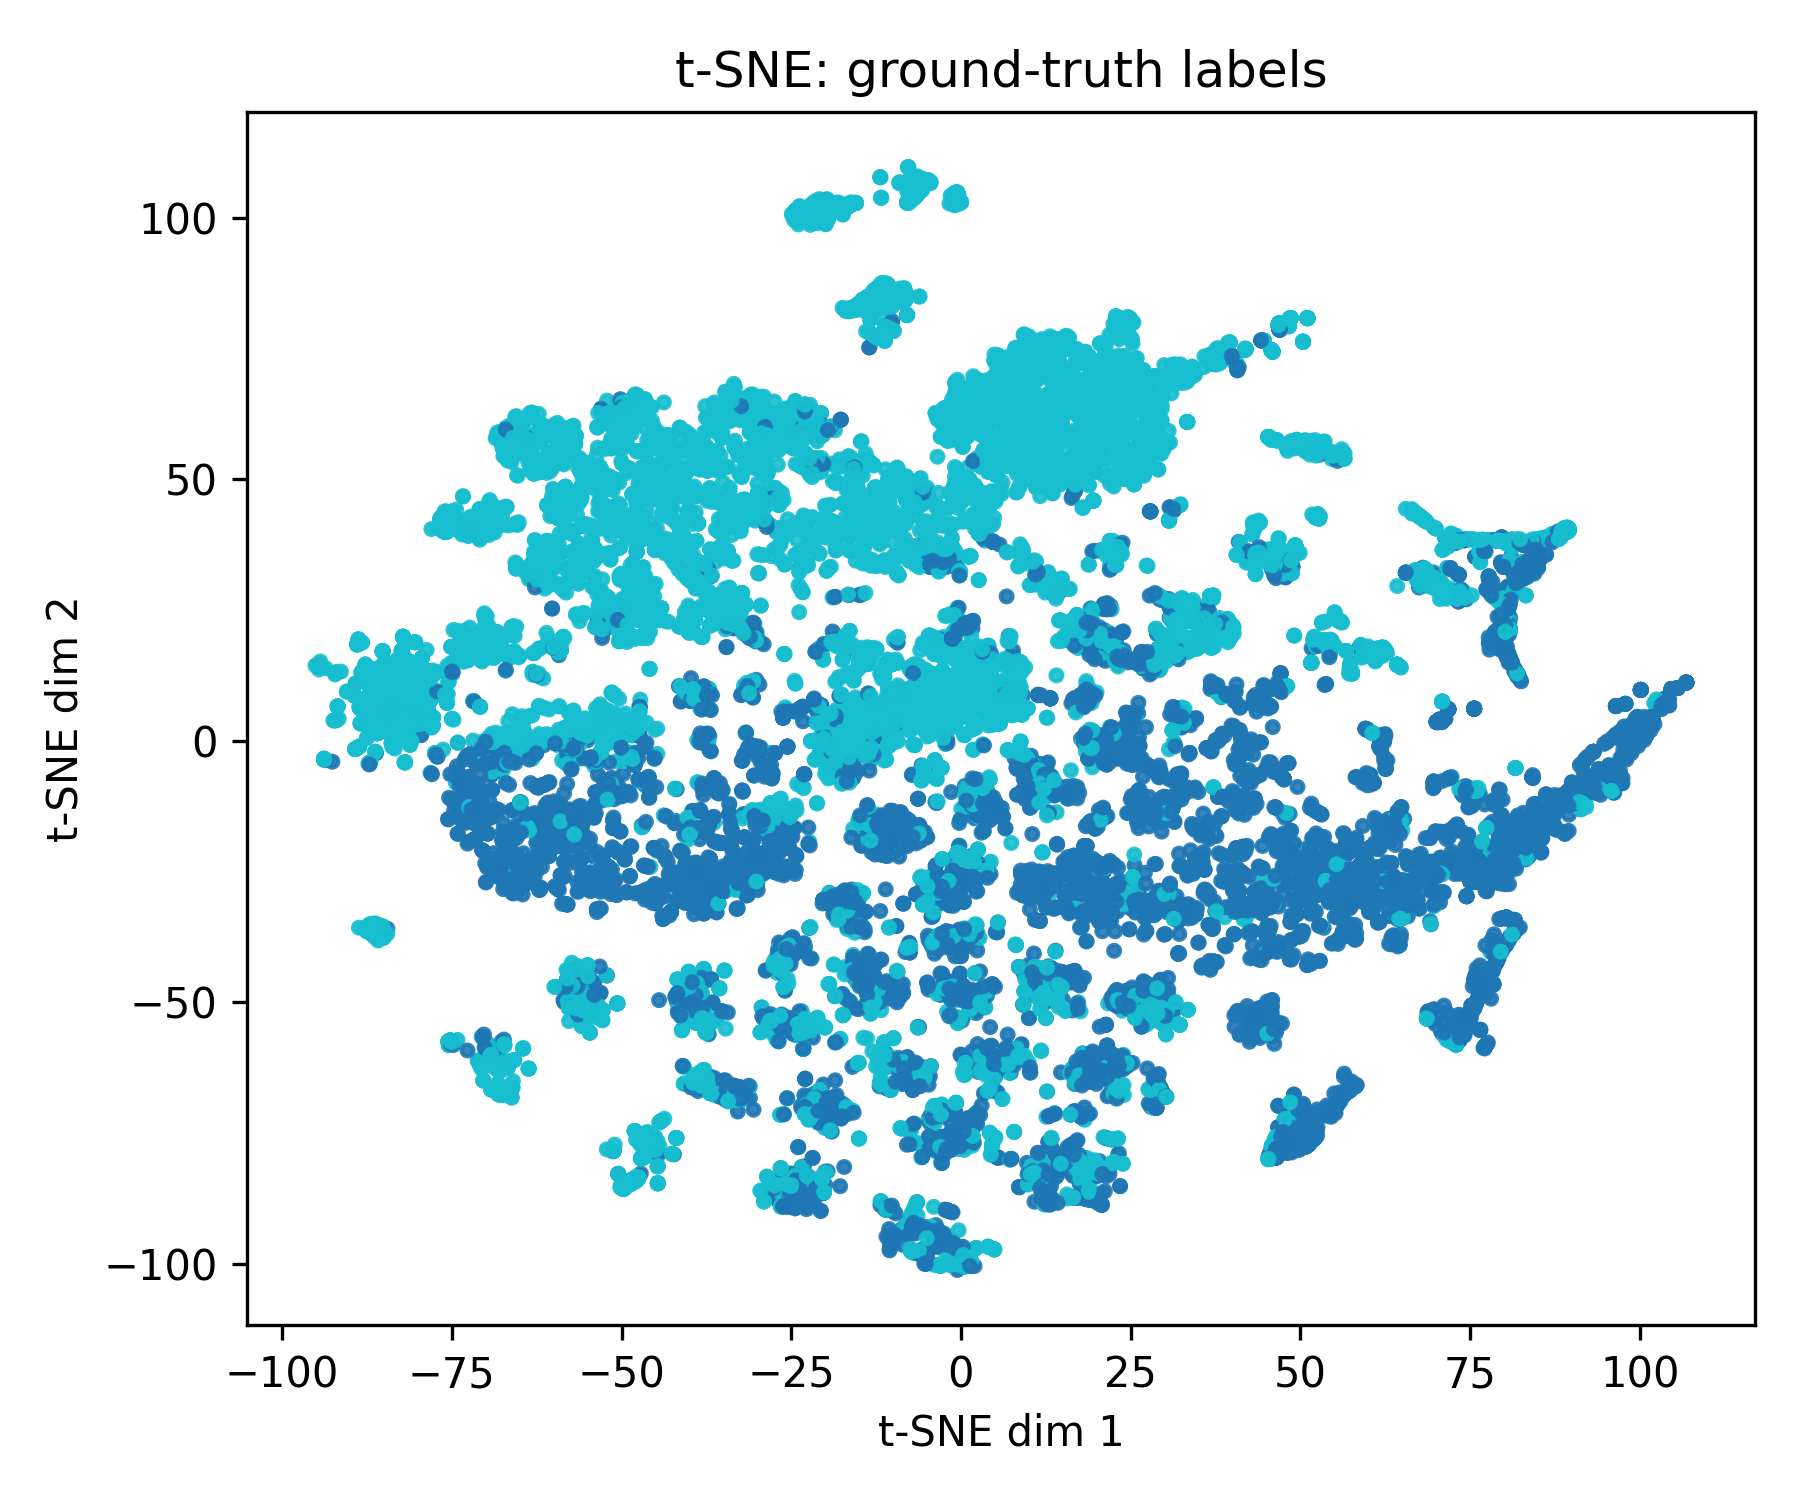
\includegraphics[width=0.45\textwidth]{tsne_ground_truth.png}
    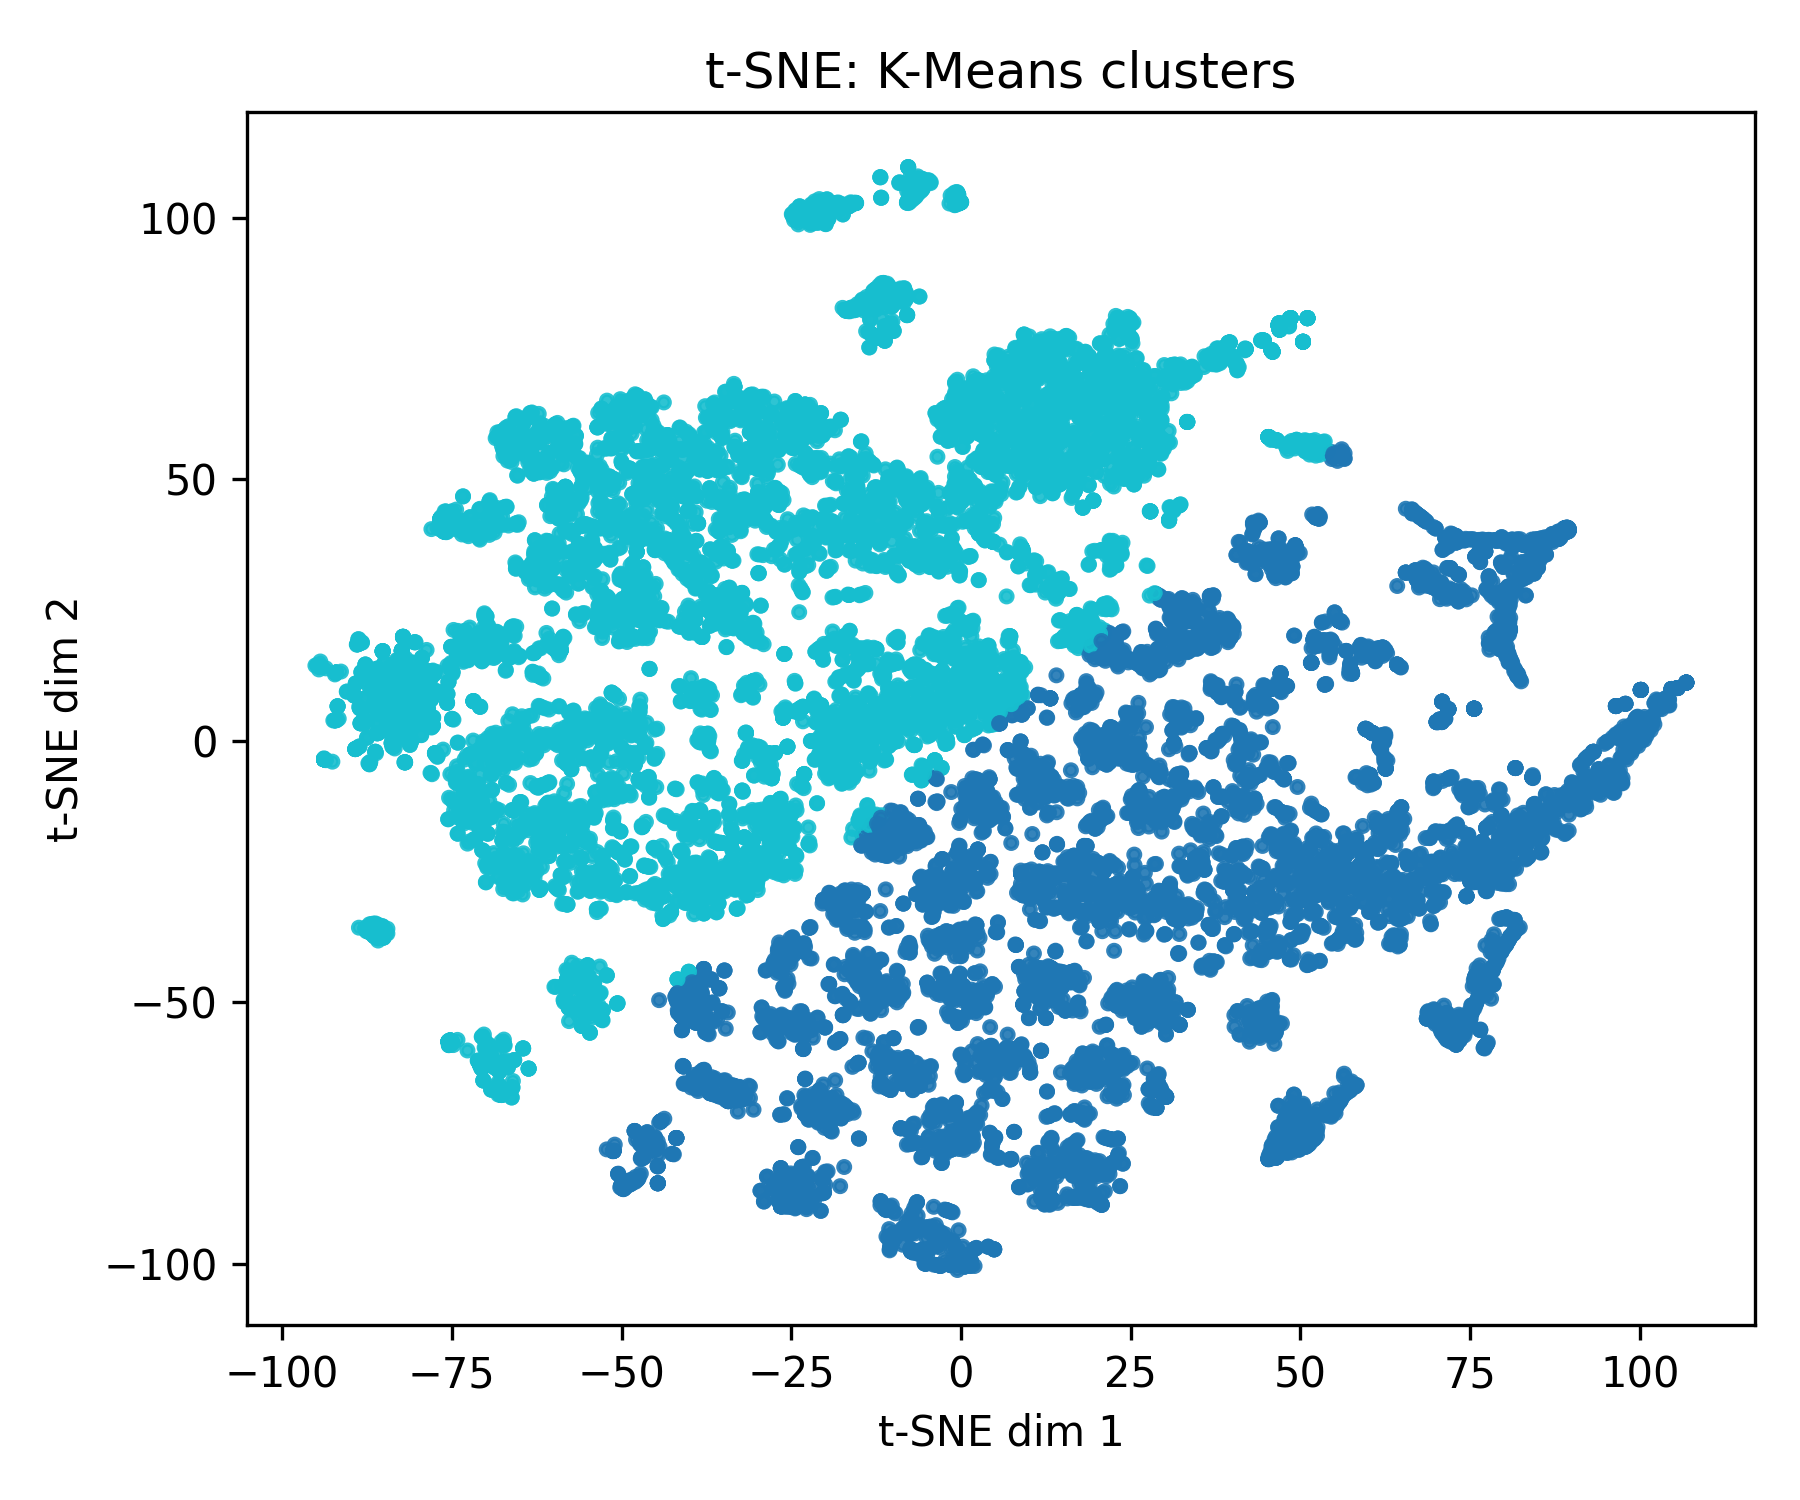
\includegraphics[width=0.45\textwidth]{tsne_kmeans.png}
    \caption{t-SNE projections of user accounts colored by (left) ground-truth labels and (right) K-Means clusters. Clear overlap suggests why unsupervised methods struggle.}
    \label{fig:tsne}
\end{figure}


Multiple unsupervised clustering methods were then applied to the reduced feature set. K-Means and Agglomerative Clustering were selected for their simplicity and effectiveness in prior bot detection research. To enhance robustness, an ensemble clustering strategy was introduced, where only accounts with consistent cluster assignments across methods were considered ``agreed'' and evaluated further.

Finally, to establish a performance baseline and validate the predictive power of the engineered features, a supervised Random Forest classifier was trained and tested using the same combined metadata and textual feature set.

\subsection{Evaluation Metrics and Results}

Clustering results were evaluated using Adjusted Rand Index (ARI), a standard metric for measuring clustering quality against ground truth labels. K-Means and Agglomerative Clustering individually achieved moderate ARI scores of 0.21 and 0.16, respectively. The ensemble clustering approach, which only considered accounts on which both methods agreed, reached an ARI of 0.20 and a classification accuracy of approximately 72\% on these agreed samples. This demonstrated that unsupervised methods could reveal meaningful structure in the data, though separation was imperfect.

\begin{figure}[ht]
    \centering
    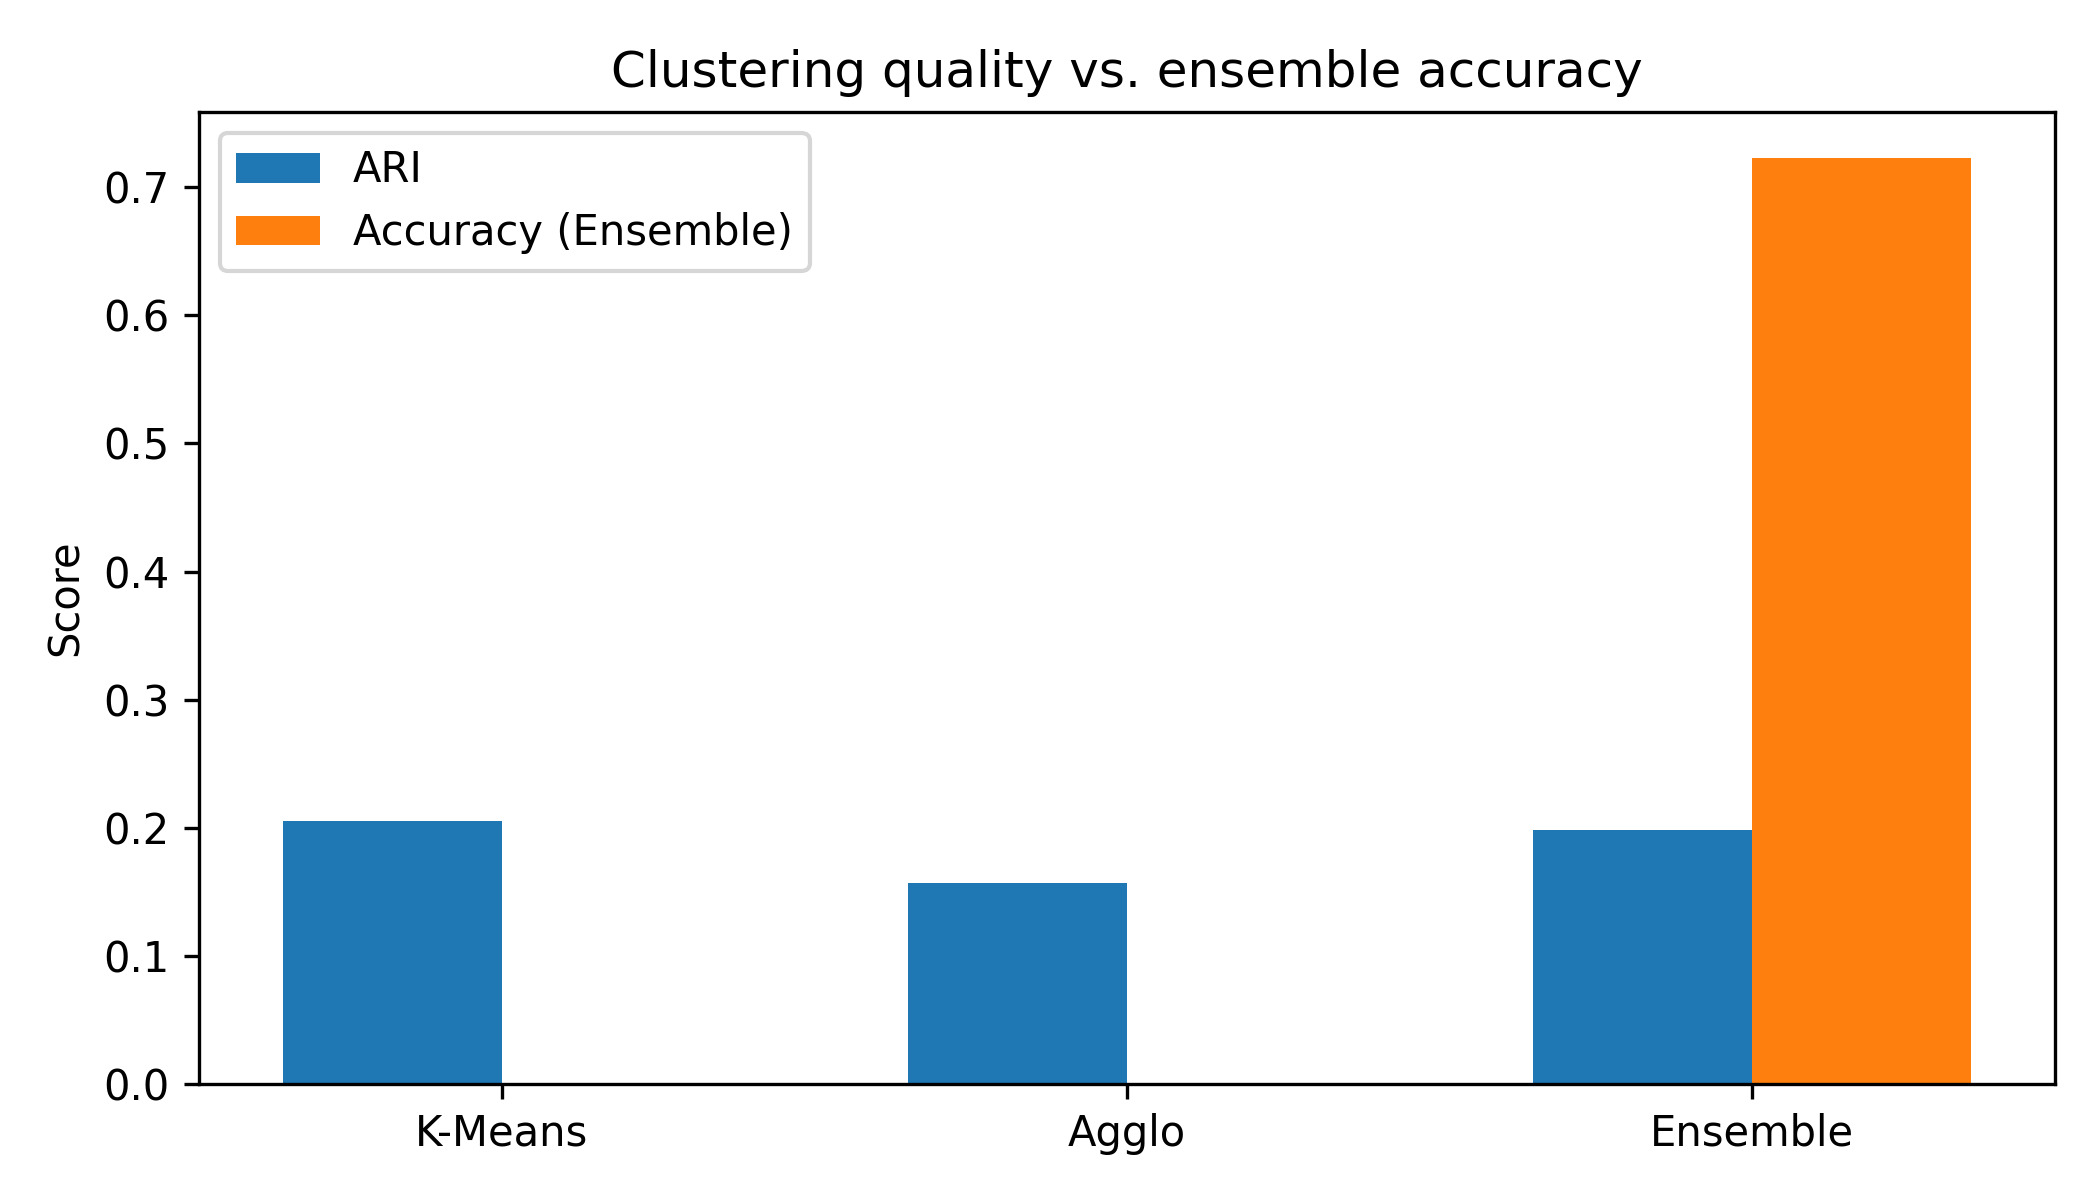
\includegraphics[width=0.48\textwidth]{clustering_metrics.png}
    \caption{Comparison of Adjusted Rand Index (ARI) across clustering algorithms, and ensemble accuracy on agreed labels.}
    \label{fig:clustering_metrics}
\end{figure}

The supervised Random Forest classifier provided a useful point of comparison. When trained on 80\% of the labeled data and evaluated on the remaining 20\%, the model achieved nearly perfect performance, with an accuracy of 99\% and precision and recall of 0.99 for both bot and human classes. This confirmed that the combined metadata and text features were highly predictive when labeled data was available.

\begin{figure}[ht]
    \centering
    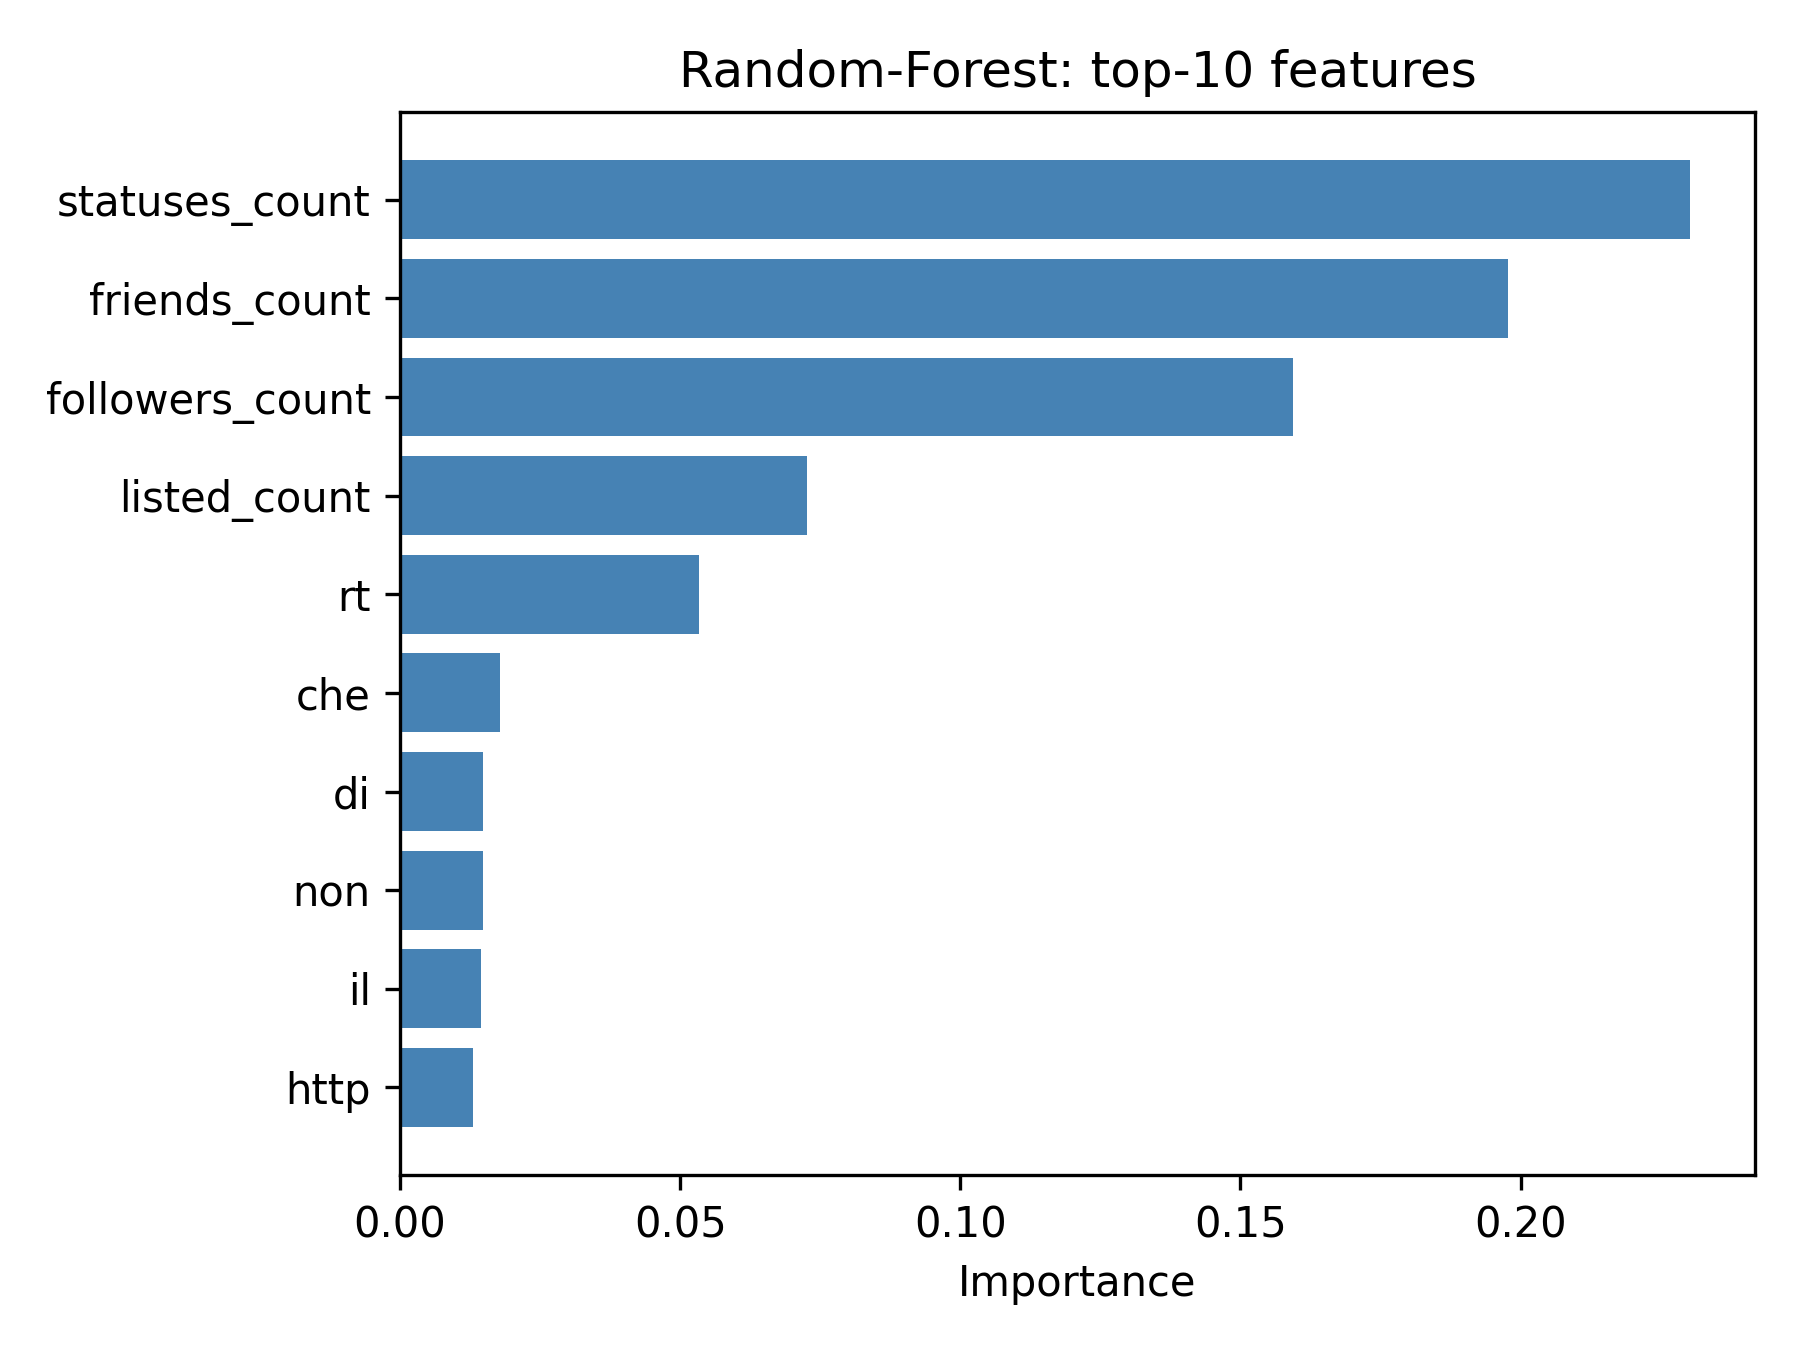
\includegraphics[width=0.48\textwidth]{rf_feature_importance.png}
    \caption{Top 10 most important features from the Random Forest classifier. Metadata dominates predictive power.}
    \label{fig:rf_importance}
\end{figure}

\subsection{Key Findings}

The results of the three-week project provided several important insights. First, unsupervised clustering alone struggled to fully distinguish between bots and humans, particularly in ambiguous cases. However, the ensemble clustering approach achieved respectable accuracy on accounts where the clustering algorithms agreed, suggesting that these methods can uncover reliably detectable patterns in a subset of the data.

Second, the supervised classification results highlighted the strength of the feature engineering pipeline. While unsupervised methods were limited, the features themselves proved highly informative, indicating that hybrid approaches — which leverage unsupervised discovery to augment or guide supervised models — hold significant promise.

These findings will shape the direction of my full comps project in the fall semester, which will focus on integrating these methods into a unified detection framework and further exploring how unsupervised insights can improve adaptability and generalization to new bot behaviors.

\section{Planned Methods and Timeline for Fall Semester}

The three-week project demonstrated both the promise and limitations of unsupervised methods for bot detection. While supervised classification achieved near-perfect accuracy, unsupervised clustering revealed meaningful patterns, especially through ensemble methods. Building on this foundation, the fall semester will focus on developing a unified framework that integrates unsupervised discovery and supervised classification to create a more flexible and interpretable bot detection system. The staged plan also aligns with the best-practice recommendations surveyed in management-oriented reviews of social-bot threats~\cite{Hajli2021social}.

\subsection{Planned Methods}

The first goal for the fall will be to expand and improve the unsupervised clustering pipeline. This will involve experimenting with advanced clustering techniques, such as DBSCAN or HDBSCAN, which can better handle noisy data and discover clusters of varying density. Additionally, I plan to refine ensemble clustering methods to improve accuracy and stability on ambiguous accounts.

Next, I will explore semi-supervised learning approaches that can leverage both labeled and unlabeled data. This may involve self-training or pseudo-labeling techniques, where confident predictions from a supervised model are iteratively used to expand the training set. This hybrid approach has the potential to improve detection of novel bots while maintaining high overall accuracy.

Beyond model development, interpretability will be a focus. By analyzing clusters and supervised model feature importances, I aim to better understand what distinguishes different types of bots, and how they differ from genuine users. This behavioral analysis will contribute to the broader research question of whether bots fundamentally act differently across categories, including spam, disinformation, and social engineering bots.

Finally, I will integrate these methods into a single bot detection pipeline and evaluate its performance. This will include thorough testing on holdout data and documentation of results for my final comps paper and presentation.

\subsection{Tentative Timeline}

\begin{itemize}
    \item \textbf{Summer (pre-semester):}  Survey advanced clustering and semi-supervised literature; create repo and data pipelines; prototype HDBSCAN and pseudo-labeling utilities.

    \item \textbf{Weeks 1--3:} Address proposal feedback; port Cresci data to the new pipeline; implement and benchmark DBSCAN \& HDBSCAN; compare to baseline K-Means.

    \item \textbf{Weeks 4--5:} Design an ensemble framework (majority vote / confidence weighting) that blends clustering outputs; tune hyper-parameters on a validation split.

    \item \textbf{Weeks 6--7:} Build a semi-supervised loop (self-training + pseudo-labels) driven by the ensemble’s high-confidence predictions; monitor label drift and class balance.

    \item \textbf{Weeks 8--9:} Conduct feature-importance and cluster-coherence analysis; visualize exemplar accounts and refine interpretability tooling.

    \item \textbf{Weeks 10--11:} Integrate unsupervised, semi-supervised, and a refreshed Random Forest into a single detection pipeline; run full hold-out evaluation.

    \item \textbf{Weeks 12--13:} Stress-test on auxiliary datasets (e.g., newer AI-generated bot data), document failure modes and ethical safeguards, and iterate on model tuning.

    \item \textbf{Week 14:} Revise final comps paper, polish figures, and rehearse presentation.
\end{itemize}


\subsection{Skills and Learning Plan}

I am already comfortable with Python, scikit-learn, and pandas, which were used extensively during the three-week project. I also have experience with basic clustering algorithms (K-Means, Agglomerative) and classification models (Random Forests). To succeed in the fall, I will need to deepen my understanding of advanced clustering methods (e.g., HDBSCAN), semi-supervised techniques (e.g., self-training and pseudo-labeling), and evaluation strategies for partially labeled data. I also plan to explore tools for improving model interpretability and documenting behavioral differences between user clusters. These skills will be developed through reading recent literature and hands-on implementation over the summer and early fall.


\section{Evaluation Metrics and Expected Results}

Evaluating bot detection methods requires metrics that reflect the differing nature of unsupervised and supervised learning tasks. Building on prior work in this domain~\cite{cresci2017paradigm,varol2017online,Grimme2018changing,Hayawi2023social}, I plan to employ standard metrics for clustering, semi-supervised learning, and supervised classification to assess the effectiveness of my final integrated detection pipeline.

\subsection{Unsupervised and Clustering Metrics}

For unsupervised clustering experiments, the primary evaluation metric will be \textbf{Adjusted Rand Index (ARI)}, which measures the similarity between cluster assignments and ground truth labels, adjusted for chance. This metric has been widely used in prior bot detection clustering studies~\cite{Grimme2018changing,Yang2023anatomy}, as it provides a rigorous way to evaluate clustering quality even when the number of clusters is unknown or imbalanced. Additionally, I will report \textbf{accuracy on ensemble-agreed samples}, following the approach from my three-week project. This reflects how well clustering methods can separate clear-cut cases, which is often the most actionable output in unsupervised bot detection.

\textbf{Expected thresholds:}
\begin{itemize}
    \item ARI exceeding 0.20 would be considered meaningful, as prior work has shown unsupervised bot detection to be a difficult problem~\cite{Yang2023anatomy}.
    \item Ensemble clustering accuracy exceeding 70\% would suggest strong agreement on clear cases, as demonstrated in preliminary experiments.
\end{itemize}

\subsection{Semi-supervised and Supervised Metrics}

For supervised classification and semi-supervised learning experiments, I will use standard classification metrics:
\begin{itemize}
    \item \textbf{Accuracy}, which captures overall correctness.
    \item \textbf{Precision}, \textbf{Recall}, and \textbf{F1-score} for both bot and human classes, to ensure balanced performance.
\end{itemize}

These metrics have been used extensively in bot detection research~\cite{varol2017online,Hayawi2023social,Orabi2020detection}. In particular, recall is critical to ensure that bots are not missed, while precision ensures that humans are not mistakenly flagged.

\textbf{Expected thresholds:}
\begin{itemize}
    \item Accuracy above 90\% will be the target, as previous supervised bot detection models have routinely reached this level on balanced datasets~\cite{Hayawi2023social}.
    \item Precision and Recall above 0.90 for both classes will be considered strong results, consistent with prior findings~\cite{Orabi2020detection,Kudugunta2018deep}.
\end{itemize}

\subsection{Qualitative and Interpretability Goals}

In addition to quantitative metrics, interpretability and behavioral insights will also be evaluated. By analyzing cluster compositions, example tweets, and supervised model feature importances, I aim to better understand the distinguishing characteristics of different bot types. This aspect is essential to answer higher-level questions about whether social engineering or disinformation bots exhibit unique behaviors, which has been highlighted as a limitation in prior work~\cite{cresci2017paradigm,Yang2023anatomy}.

These combined metrics will ensure that the final system is not only accurate but also insightful and adaptable, aligning with both technical and social goals of the comps project.

\subsection{Grading Thresholds and Contingency Plans}

If the integrated system delivers an \textbf{ARI below 0.10} \emph{or} a supervised \textbf{accuracy below 85\%}, the methodology will be deemed insufficient, triggering fallback work: revisiting feature engineering, swapping in density–based clustering (e.g., HDBSCAN), and tightening hyper-parameter search.  
Conversely, the following rubric will guide my internal assessment of semester outcomes:

\begin{itemize}
    \item \textbf{A (Excellent):} ARI $\ge 0.25$ \emph{and} supervised accuracy $\ge 95\%$ with Precision/Recall $\ge 0.93$ on both classes; clear behavioral clusters supported by qualitative analysis.
    \item \textbf{B (Good):} $0.20 \le$ ARI $< 0.25$ \emph{and} $90\% \le$ accuracy $< 95\%$; Precision/Recall $\ge 0.90$; clusters yield interpretable insights.
    \item \textbf{C (Satisfactory):} $0.15 \le$ ARI $< 0.20$ \emph{and} $85\% \le$ accuracy $< 90\%$; Precision/Recall $\ge 0.85$; some interpretability, but limited.
    \item \textbf{D (Marginal Pass):} ARI $< 0.15$ \emph{or} accuracy $< 85\%$, yet evidence of systematic effort and documented troubleshooting.
\end{itemize}

Achieving the \emph{A-tier} would demonstrate both strong predictive power and substantive insight into bot behavior; the \emph{C-tier} sets a minimum bar consistent with prior unsupervised benchmarks in the literature~\cite{Yang2023anatomy}. These thresholds ensure the project is evaluated on rigor, effectiveness, and interpretability alike.


\section{Ethical Considerations}

Bot detection systems, particularly those that leverage machine learning, raise important ethical considerations. As automated methods increasingly shape online discourse, ensuring fairness, transparency, and accountability is critical. This project is designed with these principles in mind, though several challenges and risks remain.

\subsection{False Positives and the Risk of Misclassification}

A primary ethical concern in bot detection is the risk of false positives, where genuine human users may be misclassified as bots. Such mistakes can have serious consequences, including wrongful suspension, shadow banning, or reputational harm~\cite{Rauchfleisch2020the}. While supervised models in this project have demonstrated high accuracy, no detection system is perfect. Past research shows that human judgment is also highly fallible in bot detection: Kenny et al.~\cite{Kenny2022duped} find that even trained participants regularly misidentify bots, raising concern that algorithmic models could encode similar blind spots. Additionally, Rauchfleisch and Kaiser~\cite{Rauchfleisch2020the} warn that most classifiers are tested only on a few datasets, which can lead to overly optimistic assumptions about their reliability across diverse contexts. 

To mitigate this risk, the proposed project places emphasis on interpretability and will stress-test its models on auxiliary datasets. By analyzing cluster compositions, example tweets, and feature importances in supervised models, I aim to provide transparent and understandable justifications for classifications.

\subsection{Bias and Dataset Representativeness}

Another ethical challenge stems from biases in datasets. The Cresci dataset, while widely used and respected~\cite{cresci2017paradigm}, may not fully represent the global spectrum of bots. Scholars such as Orabi et al.~\cite{Orabi2020detection} and Hayawi et al.~\cite{Hayawi2023social} emphasize that bias in bot detection systems is often a product of skewed data collection practices. Bots targeting different regions, languages, or political ideologies may escape detection simply because they deviate from the archetypes encoded in public datasets. This not only affects performance but could also deepen global inequities in content moderation and digital governance. Furthermore, many bots, such as those used for social engineering or sophisticated disinformation campaigns, may behave differently from the spam and political bots captured in existing datasets. As a result, models trained on this data risk reinforcing a narrow view of what constitutes a bot.  

This project addresses this limitation through unsupervised methods, which do not rely solely on pre-defined labels. Clustering and behavioral analysis may surface new or unexpected patterns, offering a partial remedy to dataset bias. However, the limitations of available data must be acknowledged, and results should be interpreted cautiously. Keeping this in mind, the auxiliary datasets used to stress test my project should come from a variety of geographic areas and potentially encompass multiple languages.

\subsection{Dual-Use and Responsible Deployment}

Bot detection technology also poses dual-use concerns. While the intended goal is to improve platform integrity and reduce malicious automation, such systems could be repurposed to target dissidents, activists, or other vulnerable groups. Several recent studies highlight this danger: Adams~\cite{Adams2017ai} and Yu et al.~\cite{Yu2024the} both warn that as detection tools grow more powerful, so too does their capacity for abuse, particularly by authoritarian regimes or private actors with conflicting interests. Hajli et al.~\cite{Hajli2021social} also argue that without careful oversight, bot detection infrastructure may be used to suppress unpopular speech under the guise of spam filtering or bot removal.

Given this risk, any detection system developed through this project is intended solely for research purposes and will not be deployed without further ethical review.

\subsection{Commitment to Ongoing Ethical Reflection}

Given the complexity of online environments and evolving bot strategies, no detection system can guarantee perfect fairness or neutrality. This project embraces the need for ongoing reflection and critique. Ethical considerations will continue to guide both the technical design and the interpretation of results, particularly as the project transitions into more advanced detection and behavioral analysis in the fall semester.

In line with current best practices in responsible ML development, I will also engage in iterative self-evaluation as new techniques are introduced, drawing on frameworks from applied ethics and human-centered design. The final project paper will include an ethics section detailing any unresolved concerns related to fairness, generalizability, and user harm.

\printbibliography

\end{document}
